
\section{3 lepton training for bump search testing}

\begin{figure}[H]
    \centering
    \begin{subfigure}{.45\textwidth}
        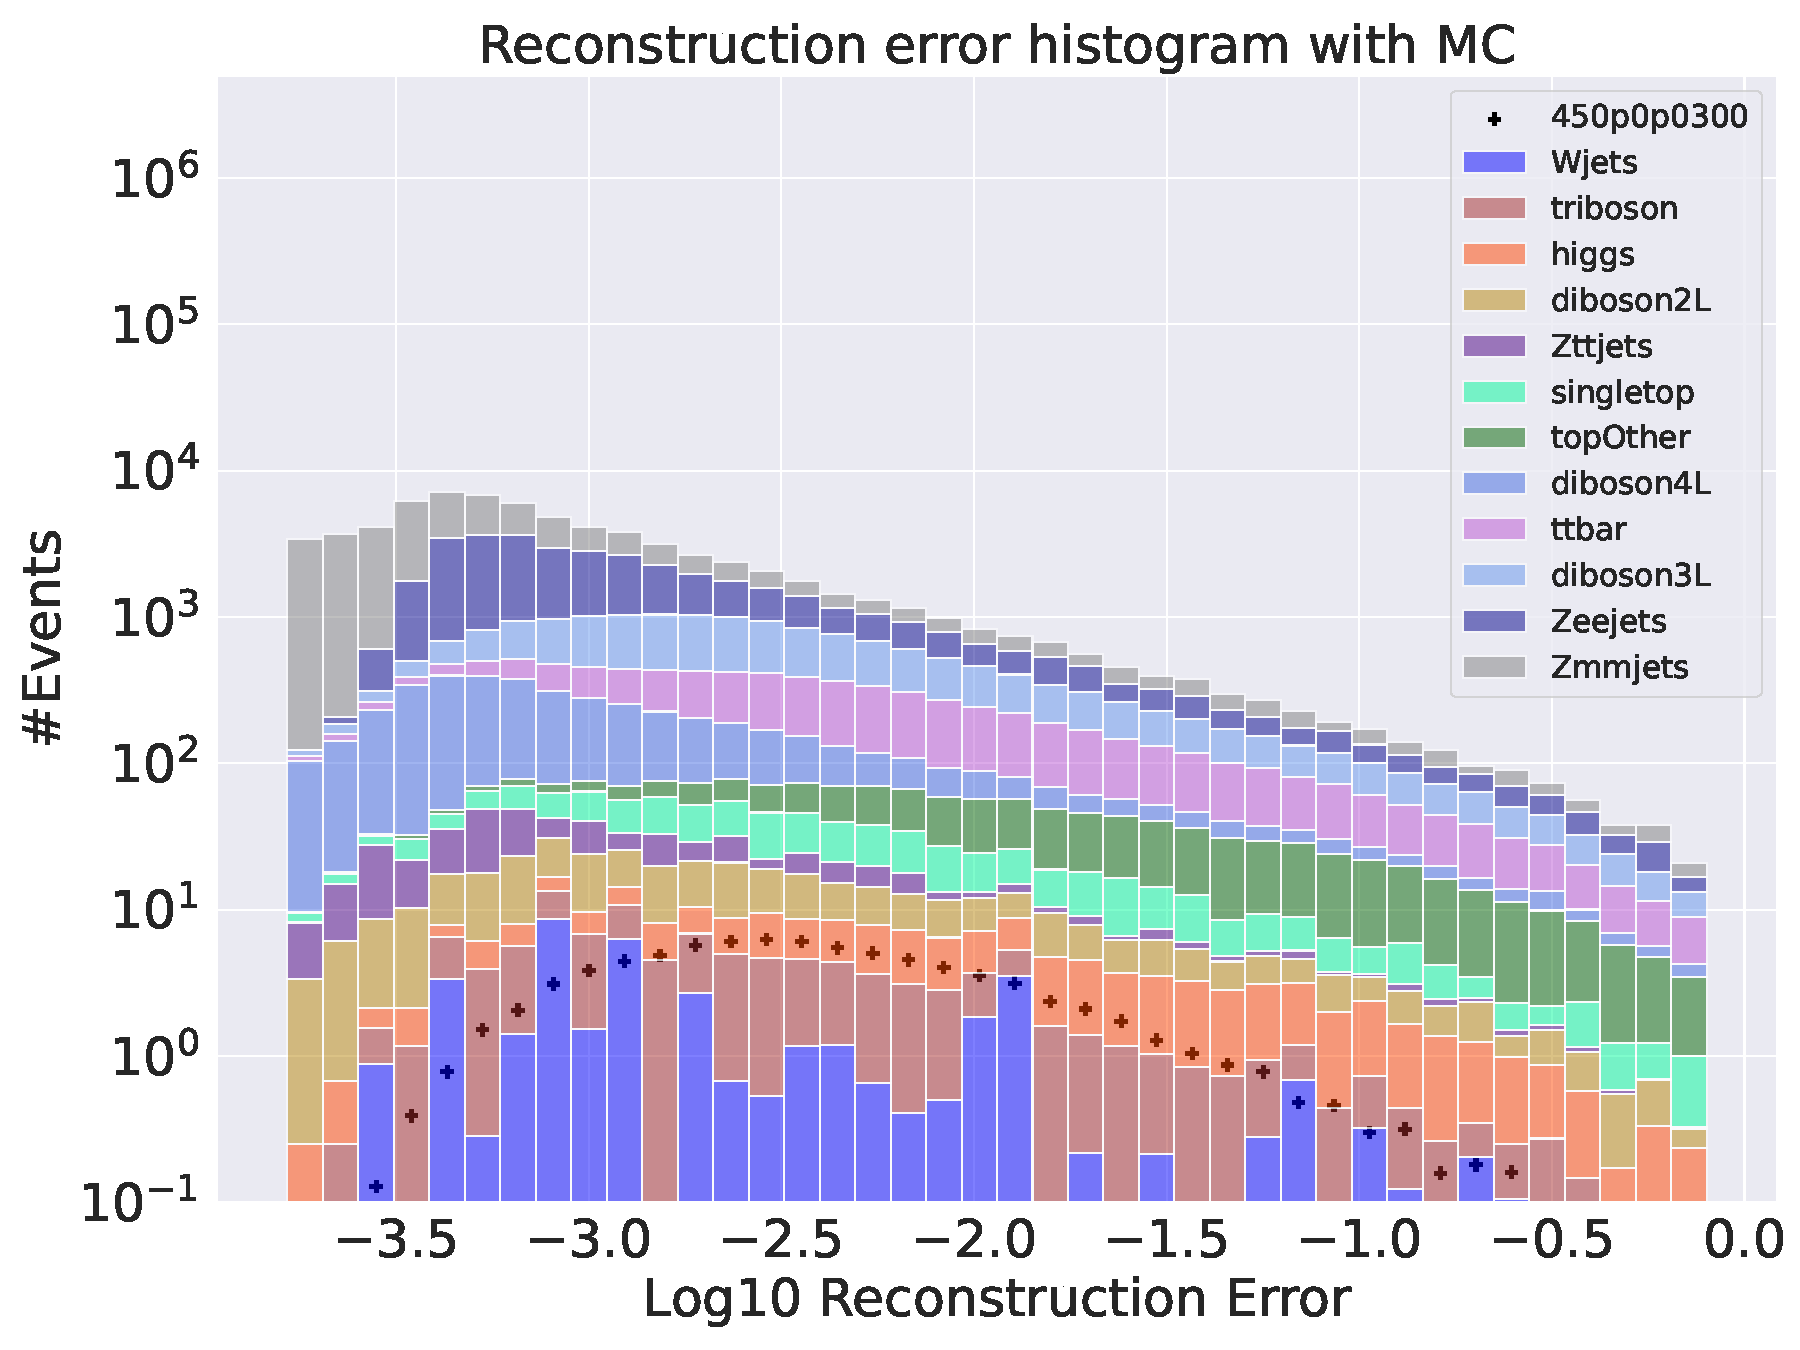
\includegraphics[width=\textwidth]{Figures/AE_testing/big/3lep/b_data_recon_big_rm3_feats_sig_450p0p0300.pdf}
        \caption{ }
        \label{fig:AE_3lep_big_450}
    \end{subfigure}
    \hfill
    \begin{subfigure}{.45\textwidth}
        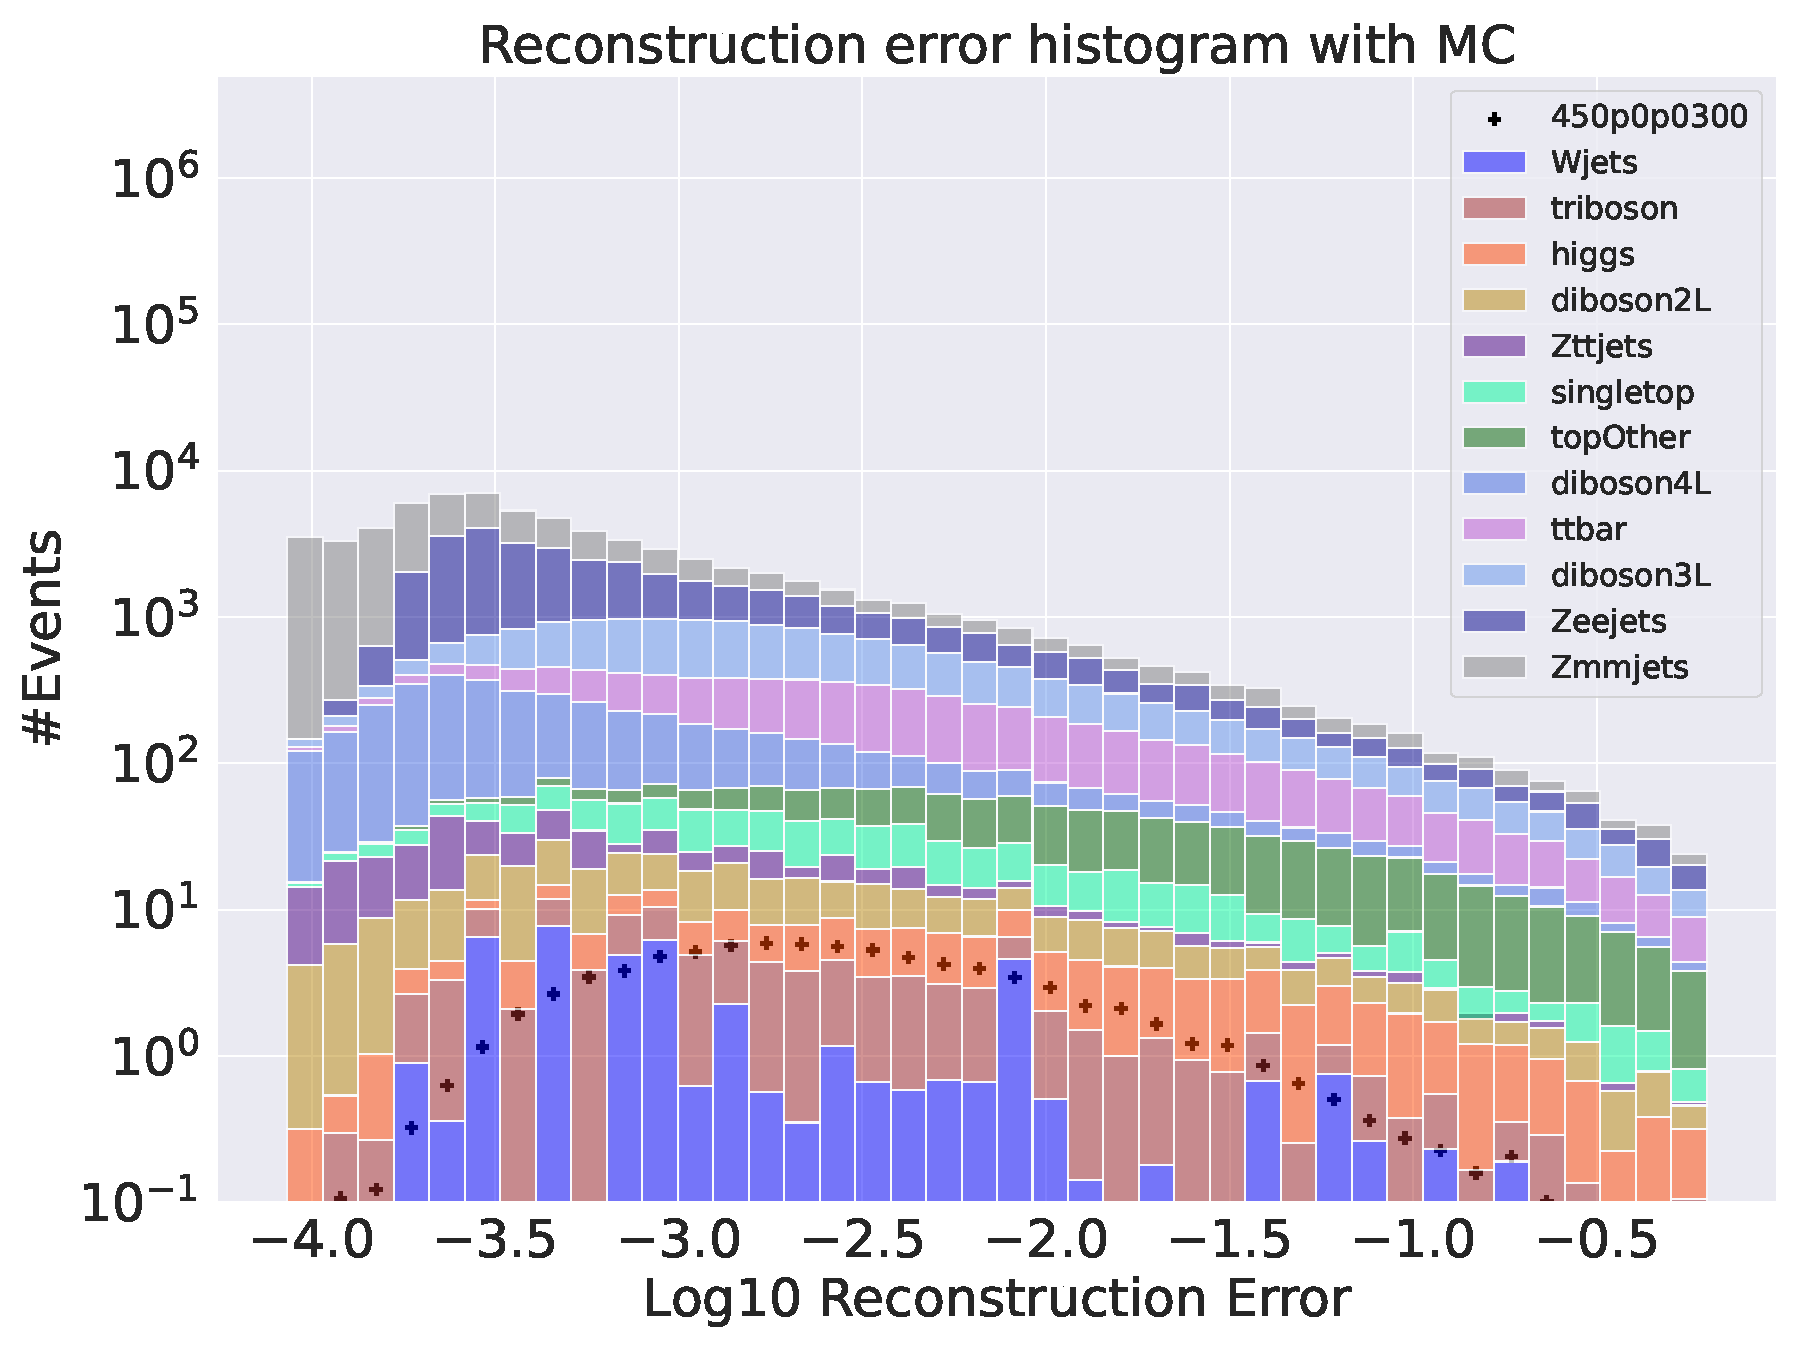
\includegraphics[width=\textwidth]{Figures/AE_testing/small/3lep/b_data_recon_big_rm3_feats_sig_450p0p0300.pdf}
        \caption{}
        \label{fig:AE_3lep_small_450}
    \end{subfigure}
    \hfill
    \begin{subfigure}{.45\textwidth}
        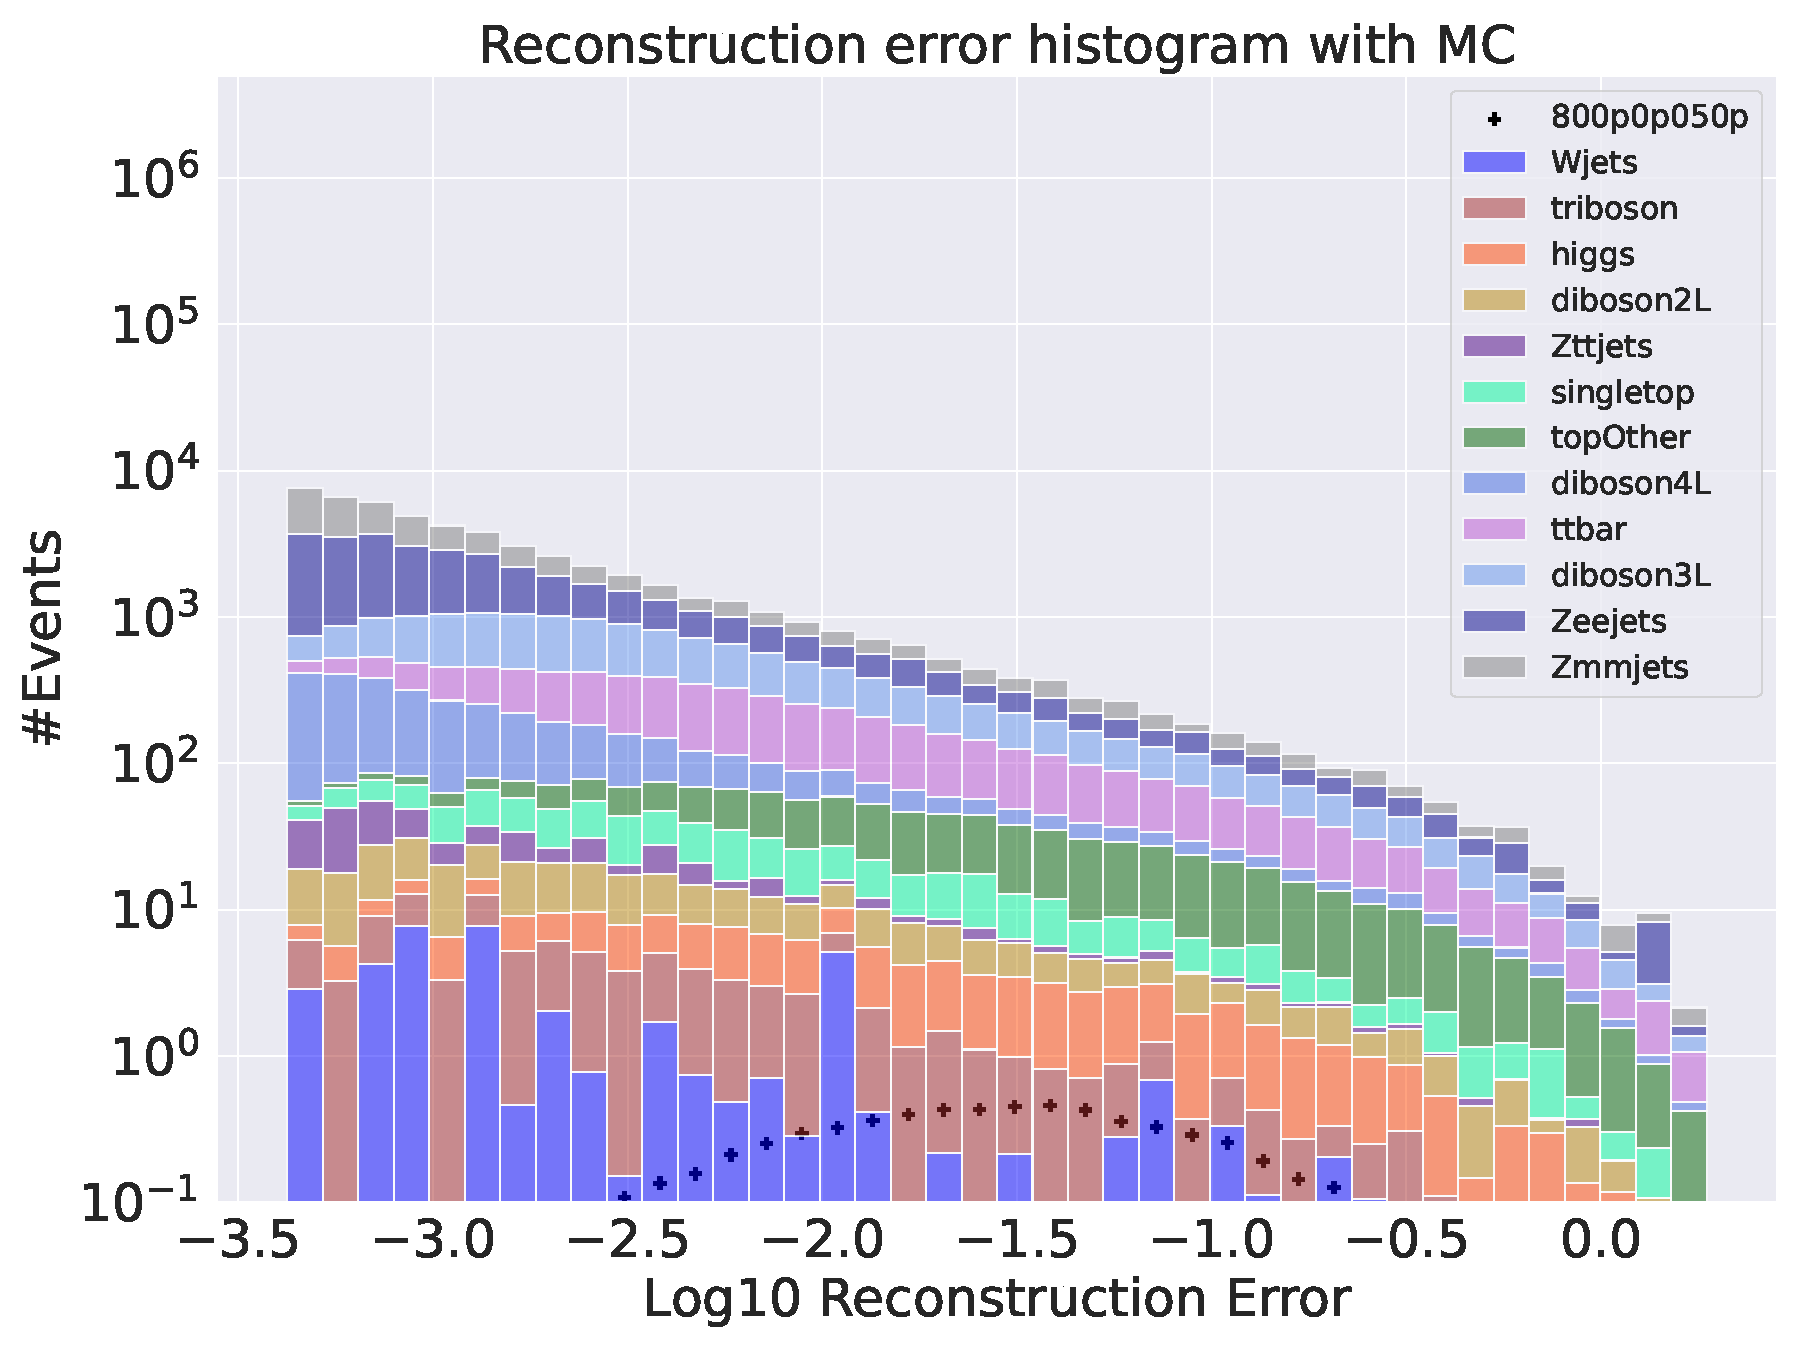
\includegraphics[width=\textwidth]{Figures/AE_testing/big/3lep/b_data_recon_big_rm3_feats_sig_800p0p050p.pdf}
        \caption{}
        \label{fig:AE_3lep_big_800}
    \end{subfigure}
    \hfill   
    \begin{subfigure}{.45\textwidth}
        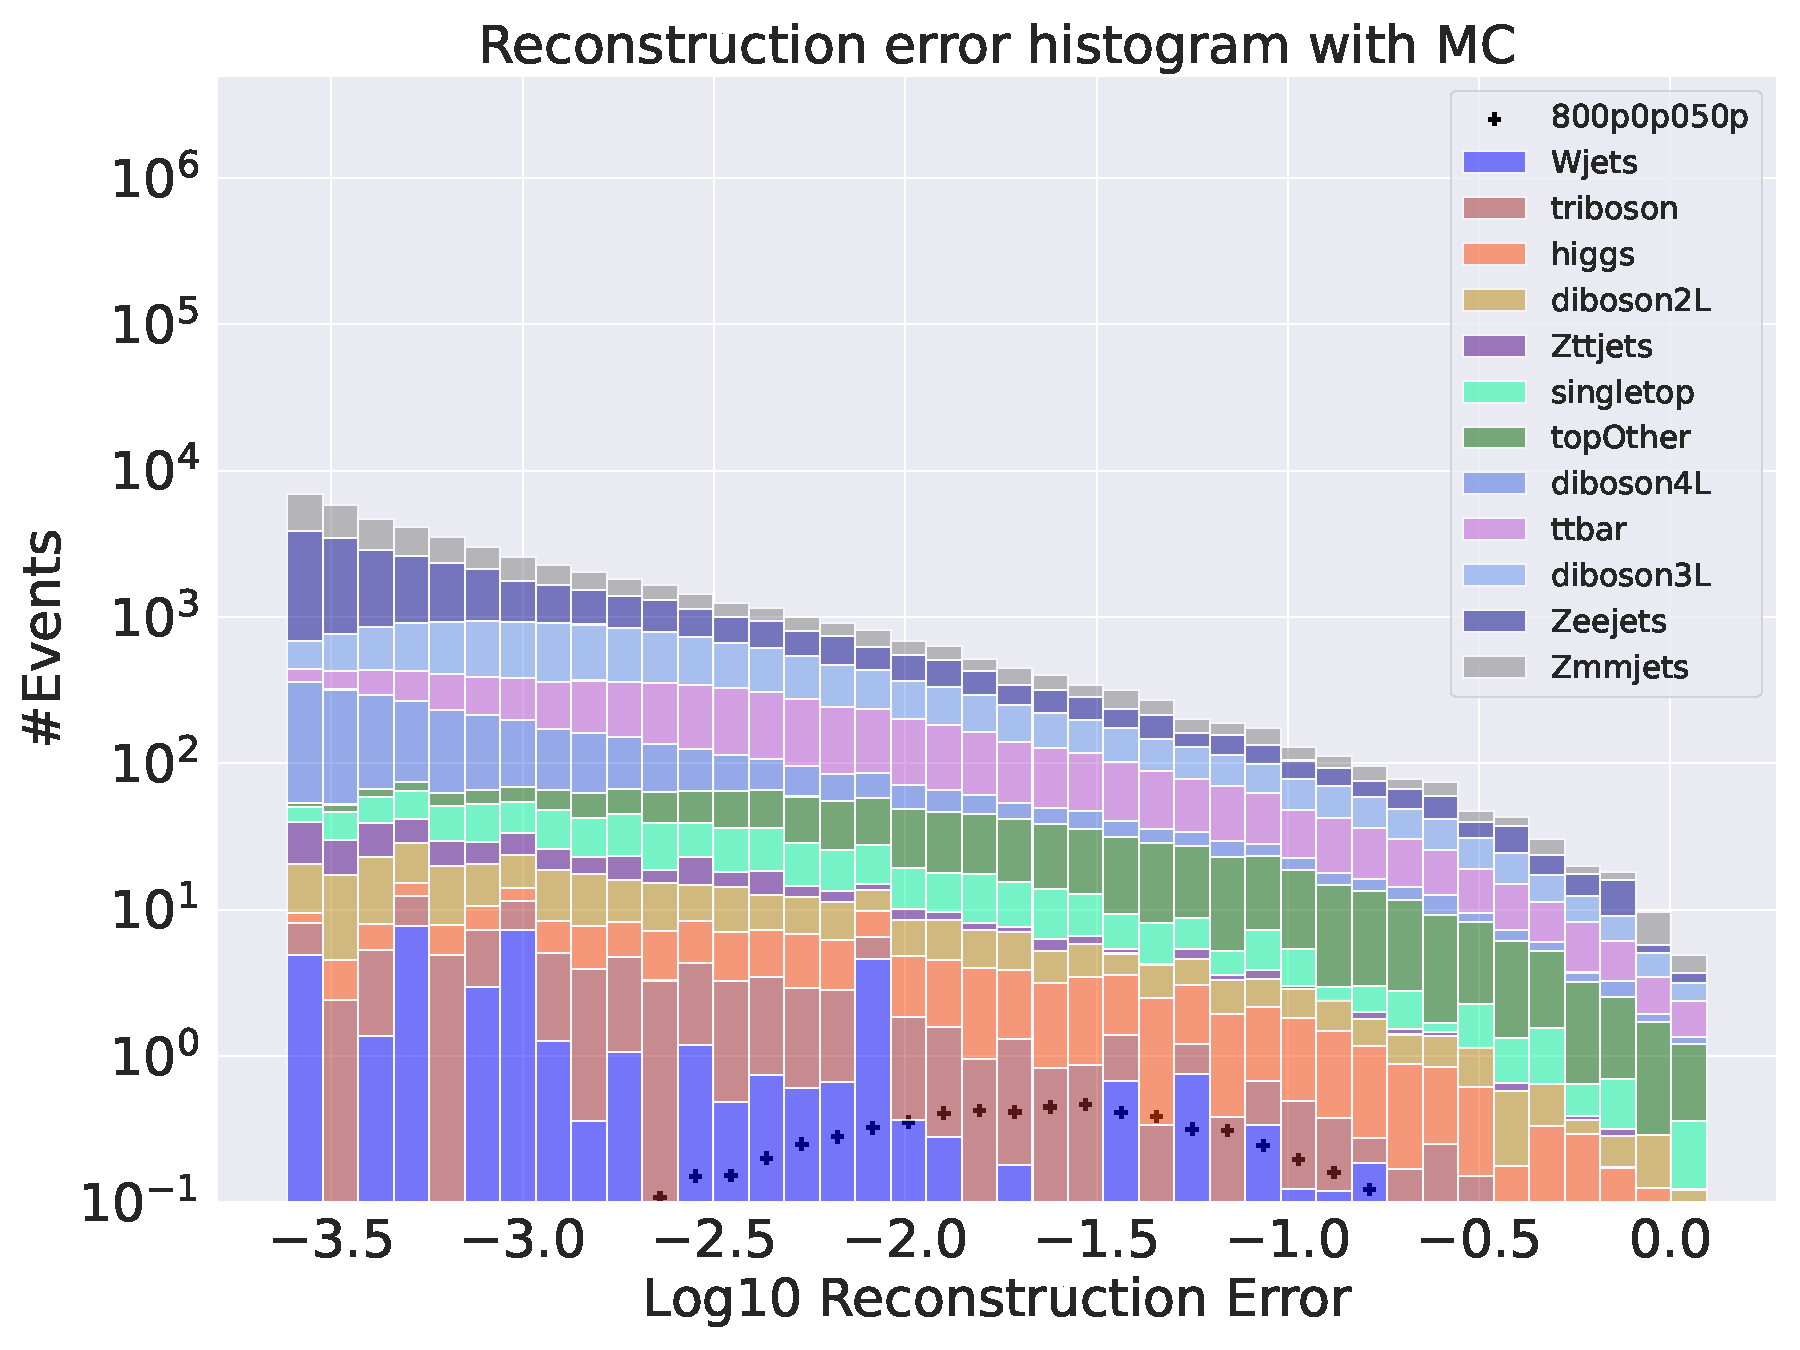
\includegraphics[width=\textwidth]{Figures/AE_testing/small/3lep/b_data_recon_big_rm3_feats_sig_800p0p050p.pdf}
        \caption{}
        \label{fig:AE_3lep_small_800}
    \end{subfigure}
    \hfill      
    \caption[3lep reconstruction error with SUSY signals for AE]{Reconstruction error distribution for the small (left) and large (right)
    regular autoencoder, using the 3 lepton + $e_T^{miss}$ dataset as training and test set. The signals used are 3 lepton + $e_T^{miss}$ 
    finalstate SUSY signals. Figures \ref{fig:AE_3lep_big_450} and \ref{fig:AE_3lep_small_450} shows the SUSY 450 and 300 mass signal, 
    and figures \ref{fig:AE_3lep_big_800} and \ref{fig:AE_3lep_small_800} shows the SUSY 800 and 50 mass signal.}
    \label{fig:AE_3lep_recon_err_both_sig}
\end{figure}


